\chapter{Escopo de Projeto}


O painel de LED pode descrito equipamentos concebidos com o objetivo de receber dados de uma fonte externa fornecendo dados de saída como reprodução de imagens (item 3.3.4 (c) NBR5410:2004), deste modo, ele pode ser classificado como equipamento de tecnologia da informação (ETI).
elaboração e dimensionamento de quadro de distribuição elétrica dedicados a fornecer energia para paineis Full Led com tensão de 127/220V e 220/380 V.


 
\section{Potência dos Modelos de Paineis Full Color}
%tabela com as potências e tamanho de cada modelo
A entrada de energia de cada gabinete é realizado através de fontes de energia. As especifiações de entrada.
\begin{table}[htbp]
\caption{}
\centering
\begin{tabular}{ l c c c c}
\toprule
\multirow{2}{*}{Modelo}& Gabinetes       & 	 		 \multicolumn{3}{c}{Potência (W)} 			 \\ 
\cmidrule{3-5}
                       & Qnt   & \multicolumn{1}{c}{P10} & \multicolumn{1}{c}{P5} & \multicolumn{1}{c}{P8} \\ 
\midrule

Painel 2 X 2           & 4      & 2160 			    & 2736 			& 2520 \\ 
Painel 2 X 3           & 6      & 3240 				& 4104 			& 3780 \\ 
Painel 3 X 2           & 6      & 3240 				& 4104 			& 3780 \\ 
Painel 3 X 3           & 9      & 4860 				& 6156 			& 5670 \\ 
Painel 4 X 2           & 8      & 4320 				& 5472 			& 5040 \\ 
Painel 4 X 3           & 12     & 6480 				& 8208 			& 7560 \\ 
Painel 4 X 4           & 16     & 8640 				& 10944 		& 10080 \\
Painel 5 X 2		 & 10 		& 5400 				& 6840 			& 6300 \\ 
Painel 5 X 3 			& 15 	& 8100 				& 10260 		& 9450 \\
Painel 6 X 2 			& 12 	& 6480 				& 8208 			& 7560 \\ 
Painel 7 X 3 			& 21 	& 11340 			& 14364 		& 13230 \\ 
Painel 9 X 3 			& 27 	& 14580 			& 18468 		& 17010 \\ 
Painel 10 X 4 			& 40 	& 21600 			& 27360 		& 25200 \\
\bottomrule
\end{tabular}
\label{tab:pot_Painel}
\end{table}

 
\section{Tecnologia de iluminação LED}
Existe algumas caracteristicas da tecnologia LED que devemos ter atenção. Tal como alguns potenciais restrições que poderemos ter que superar.
\begin{itemize}
\item Corrente de pico potencialmente muito elevada ao ligar.
\item Geração de poluição hamonica
\item Temperatura elevada nas conexões
\item Radiação no espectro azul
\item Piscar quando desligada.
\end{itemize}

Ao ligar uma luminária LED ocorre uma corrente variavel durante o primeiro segundo, a corrente se estabiliza quando atinge a condição de operação nominal. Na partida da luminária pode ser identificado três estados transitórios:
\begin{itemize}
  \item Estado 1: Corrente de pico.
  \item Estado 2: inicialização do driver.
  \item Estado 3: Alimentando a carga LED.
  \end{itemize}  
O estado 4 correponde a condição de operação estacionário. Este estados estão numerados na figura.
\begin{figure}[h]
    \centering
    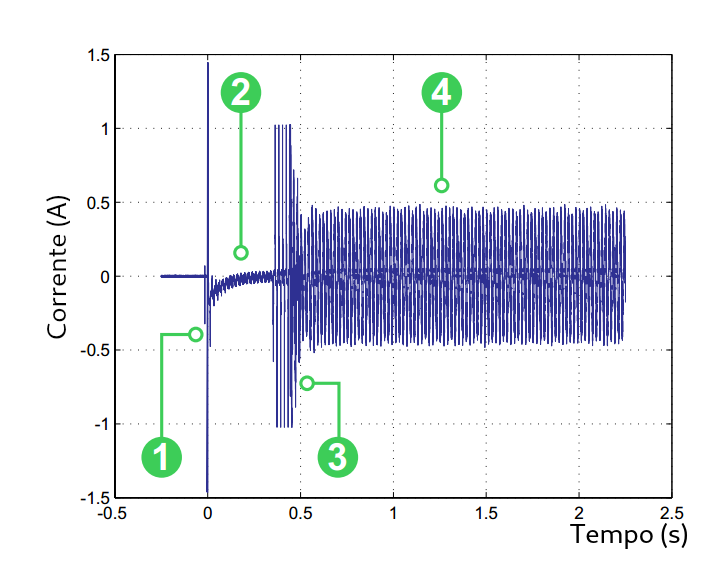
\includegraphics[width=0.6\textwidth]{image/correntextempo.png}
    %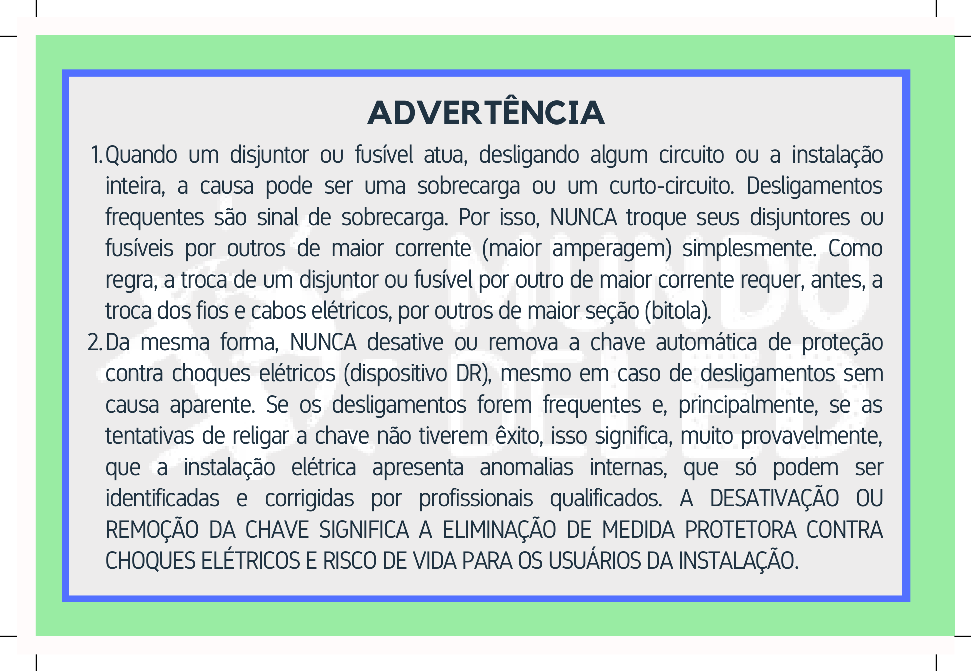
\includegraphics[width=4cm]{image/EtiqAdvQD.pdf}
    \caption{Gráfico Corrente x tempo, da partida de luminária LED retirada}
   \label{fig:bornes}
\end{figure}
Esta caracteristica influencia na escolha do disjuntor. 

\section{Influências externas}

Condições exterior a que o quadro terminal possam estar sujeitos.
Temperatura ambiente
grau de proteção

\section{Tipos de Quadro Terminal}

Existem proteções básicas e obrigatórios segundo as normas, e a proteção mais especifica que podem ser necessárias devido a influências externas, tal como, sensibilidade de equipamento devido a oscilação da rede, partida de motores de indução, etc.
\begin{description}
\item[Obrigatórios] Proteção contra sobrecorrente. Protege contra incêndios, contra sobrecarga e contra curto circuito. Dispositivo utilizado disjuntor.
\item[obrigatório em áreas úmidas] Proteção contra fuga a Terra. Protege contra
\end{description}

No geral um quadro de distribuição elétrica contém:
\begin{list}{•}{•}
\item Dispositivos de proteção: disjuntores termomagnéticos (DTM), interruptores diferenciais (IDR) e dispositivo de proteção contra surtos(DPS);
\item Barramentos de inteligação das fases;
\item Barramento de neutro;
\item Barramento de proteção PE (terra);
\\item Estrutura: composta de caixa metálica, chapa de montagem dos componentes, isoladores, tampa(espelho) e porta com dobradiça.
\end{list}

Para nomear os quadros vamos utilizar o seguinte padrão de código:
\begin{table}[!h]
\begin{tabular}{c  c c l  l l l r l l}
Quadro 		& l x c		& 	 &{y}			& 		&{Pn}			& 			&{yyyV} 	&			&\\

			& 	\vline	& 	  & 	\vline	&		&		\vline	&			&	\vline 		& 	&	Tensão (F-N) 127; 220;  \\
\cline{9-10} 
			& 	\vline	& 	  & 	\vline	&		&		\vline	&			&			&			&	Led 5, 8 ou 10;  \\
\cline{7-10} 
			& 	\vline	& 	  & 	\vline &		&				&			&			&			&	Monofásico (M), Trifásico (T);  \\
\cline{5-10} 
			& 	\vline	& 	  & 			&		&				&			&			&			&	 Qtd gabinetes por linha(l) e coluna (c);  \\
\cline{3-10} 
\end{tabular}
%\caption{Codigo do quadro para qual painel ele serve}
\end{table}
Como exemplo um quadro terminal para o painel full led  P8 4x3 m que será instalado em uma rede com tensão fase neutro (F-N) 127 V e entre fase 220 V (F-F) no modelo trifásico, terá o seguinte código Quadro 4x3T P8 127V
\section{Parâmetros de Projeto}
Parâmetros de projeto comum para todos os quadros
\begin{itemize}
\item Parâmentros de projeto
\item Corrente de curto circuito:  xx A
\item Queda de tensão
\item Fatores de demanda considerados
\item Temperatura ambiente
\end{itemize}
   
   
A corrente de curto circuito de entrada 380V e potencia de transformador 112,5 kVA Icc 4,8 kA, fator de potência 0,7

\section{Dados do montador}
Conforme a NBR IEC 61439-1 os item declarados pelo montador do conjunto %\cite{NormasTecnicas2016}:
\begin{description}
\item[$U_{n}$] tensão nominal do CONJUTO (item 5.2.1) a tensão nominal deve ser ao menos igual à tensão nominal do sistema elétrico.

\item[$U_{e}$] tensão de utilização de um circuito. A tensão nominal de utilização não pode ser inferior à tensão nominal do sistema elétrico ao qual é previsto para ser conectado.
\item[$U_{i}$] tensão nominal de isolamento de um circuito é o valor da tensão para os quais as tensões de ensaio dielétricas e distâncias de escoamento são referidas. $U_{i} \leq U_{n} e U_{i} \leq U_{e}$

\item[$U_{imp}$] Valor de tensão de impulso suportável, caracterizando a cpacidade de suportar a isolação contra sobretensões trnasitórias especificadas. (item 3.8.9.4 da norma ABNT 61439-1 )

\item[$I_{n}$] valor de corrente que o circuito pode conduzir sem que a elevação de temperatura das diferentes partes do CONJUNTO exceda os limites especificados em condições especificas. $I_{nA}$ corrente nominal do CONJUNTO (item 5.3.1); $I_{nc}$ corrente nominal de um circuito (item 5.3.2)
\item[$I_{pk}$] valor de pico de corrente de curto-circuito, que pode ser suportado sob condições especificadas.
\item[$I_{cw}$] valor eficaz da corrente de curta duração, que o circuito pode suportar em condições especificadas, definido em termos de corrente e duração.
\item[$I_{cc}$]valor da corrente de curto-circuito presumida, que o circuito protegido por um dispositivo de proteção contra curto-circuito (DPCC)pode suportar durante o tempo total de funcionamento desse dispositivo nas condições especificadas.
\item[RDF - \textit{Rated Diversity Factor}] valor por unidade de corrente nominal, que os circuitos de saída de um CONJUNTO podem ser carregados de forma contínua e simultânea leando um consideração as influências térmicas mútuas.
\item[$f_{n}$] valor de frequência para o qual um circuito é projetado e para o qual se referem as condições de utilização.A atribuição pode ser por faixa de frequencia ou especificar se é em corrente alternada ou corrente contínua item 3.8.12


\end{description}


